\documentclass[12pt,letterpaper,leqno]{article}
\usepackage{amsmath,amsthm,amsfonts,amssymb,amscd}
\usepackage{fullpage}
\usepackage{lastpage}
\usepackage{enumerate}
\usepackage{fancyhdr}
\usepackage{mathrsfs}
\usepackage{xcolor}
\usepackage[margin=3cm]{geometry}
\setlength{\parindent}{0.0in}
\setlength{\parskip}{0.05in}
\usepackage{graphicx}
\usepackage{listings}
\lstset{
  numbers=left,
  numbersep=5pt,
  stepnumber=1,
  tabsize=2,
  showstringspaces=false
}

% Edit these as appropriate
\newcommand\course{CS570}
\newcommand\semester{Fall 2014}     % <-- current semester
\newcommand\hwnum{5}                  % <-- homework number
\newcommand\yourname{Matt Dickenson} % <-- your name
\newcommand\login{mcd31}           % <-- your NetID
\newcommand\hwdate{Due: November 25, 2014}           % <-- HW due date

\newcommand\myand{\wedge}
\newcommand\myor{\vee}
\newcommand\mynot{\neg}
\renewcommand\implies{\Rightarrow}

\newenvironment{answer}[1]{
  \subsubsection*{Problem #1}
}


\pagestyle{fancyplain}
\headheight 35pt
\lhead{\yourname\ \texttt{\login}\\\course\ --- \semester}
\chead{\textbf{\Large Homework \hwnum}}
\rhead{\hwdate}
\headsep 10pt

\begin{document}




\begin{answer}{1}

A graphical version of the MDP described in the homework is shown in Figure 1:

\begin{figure}[h!]
\begin{center}
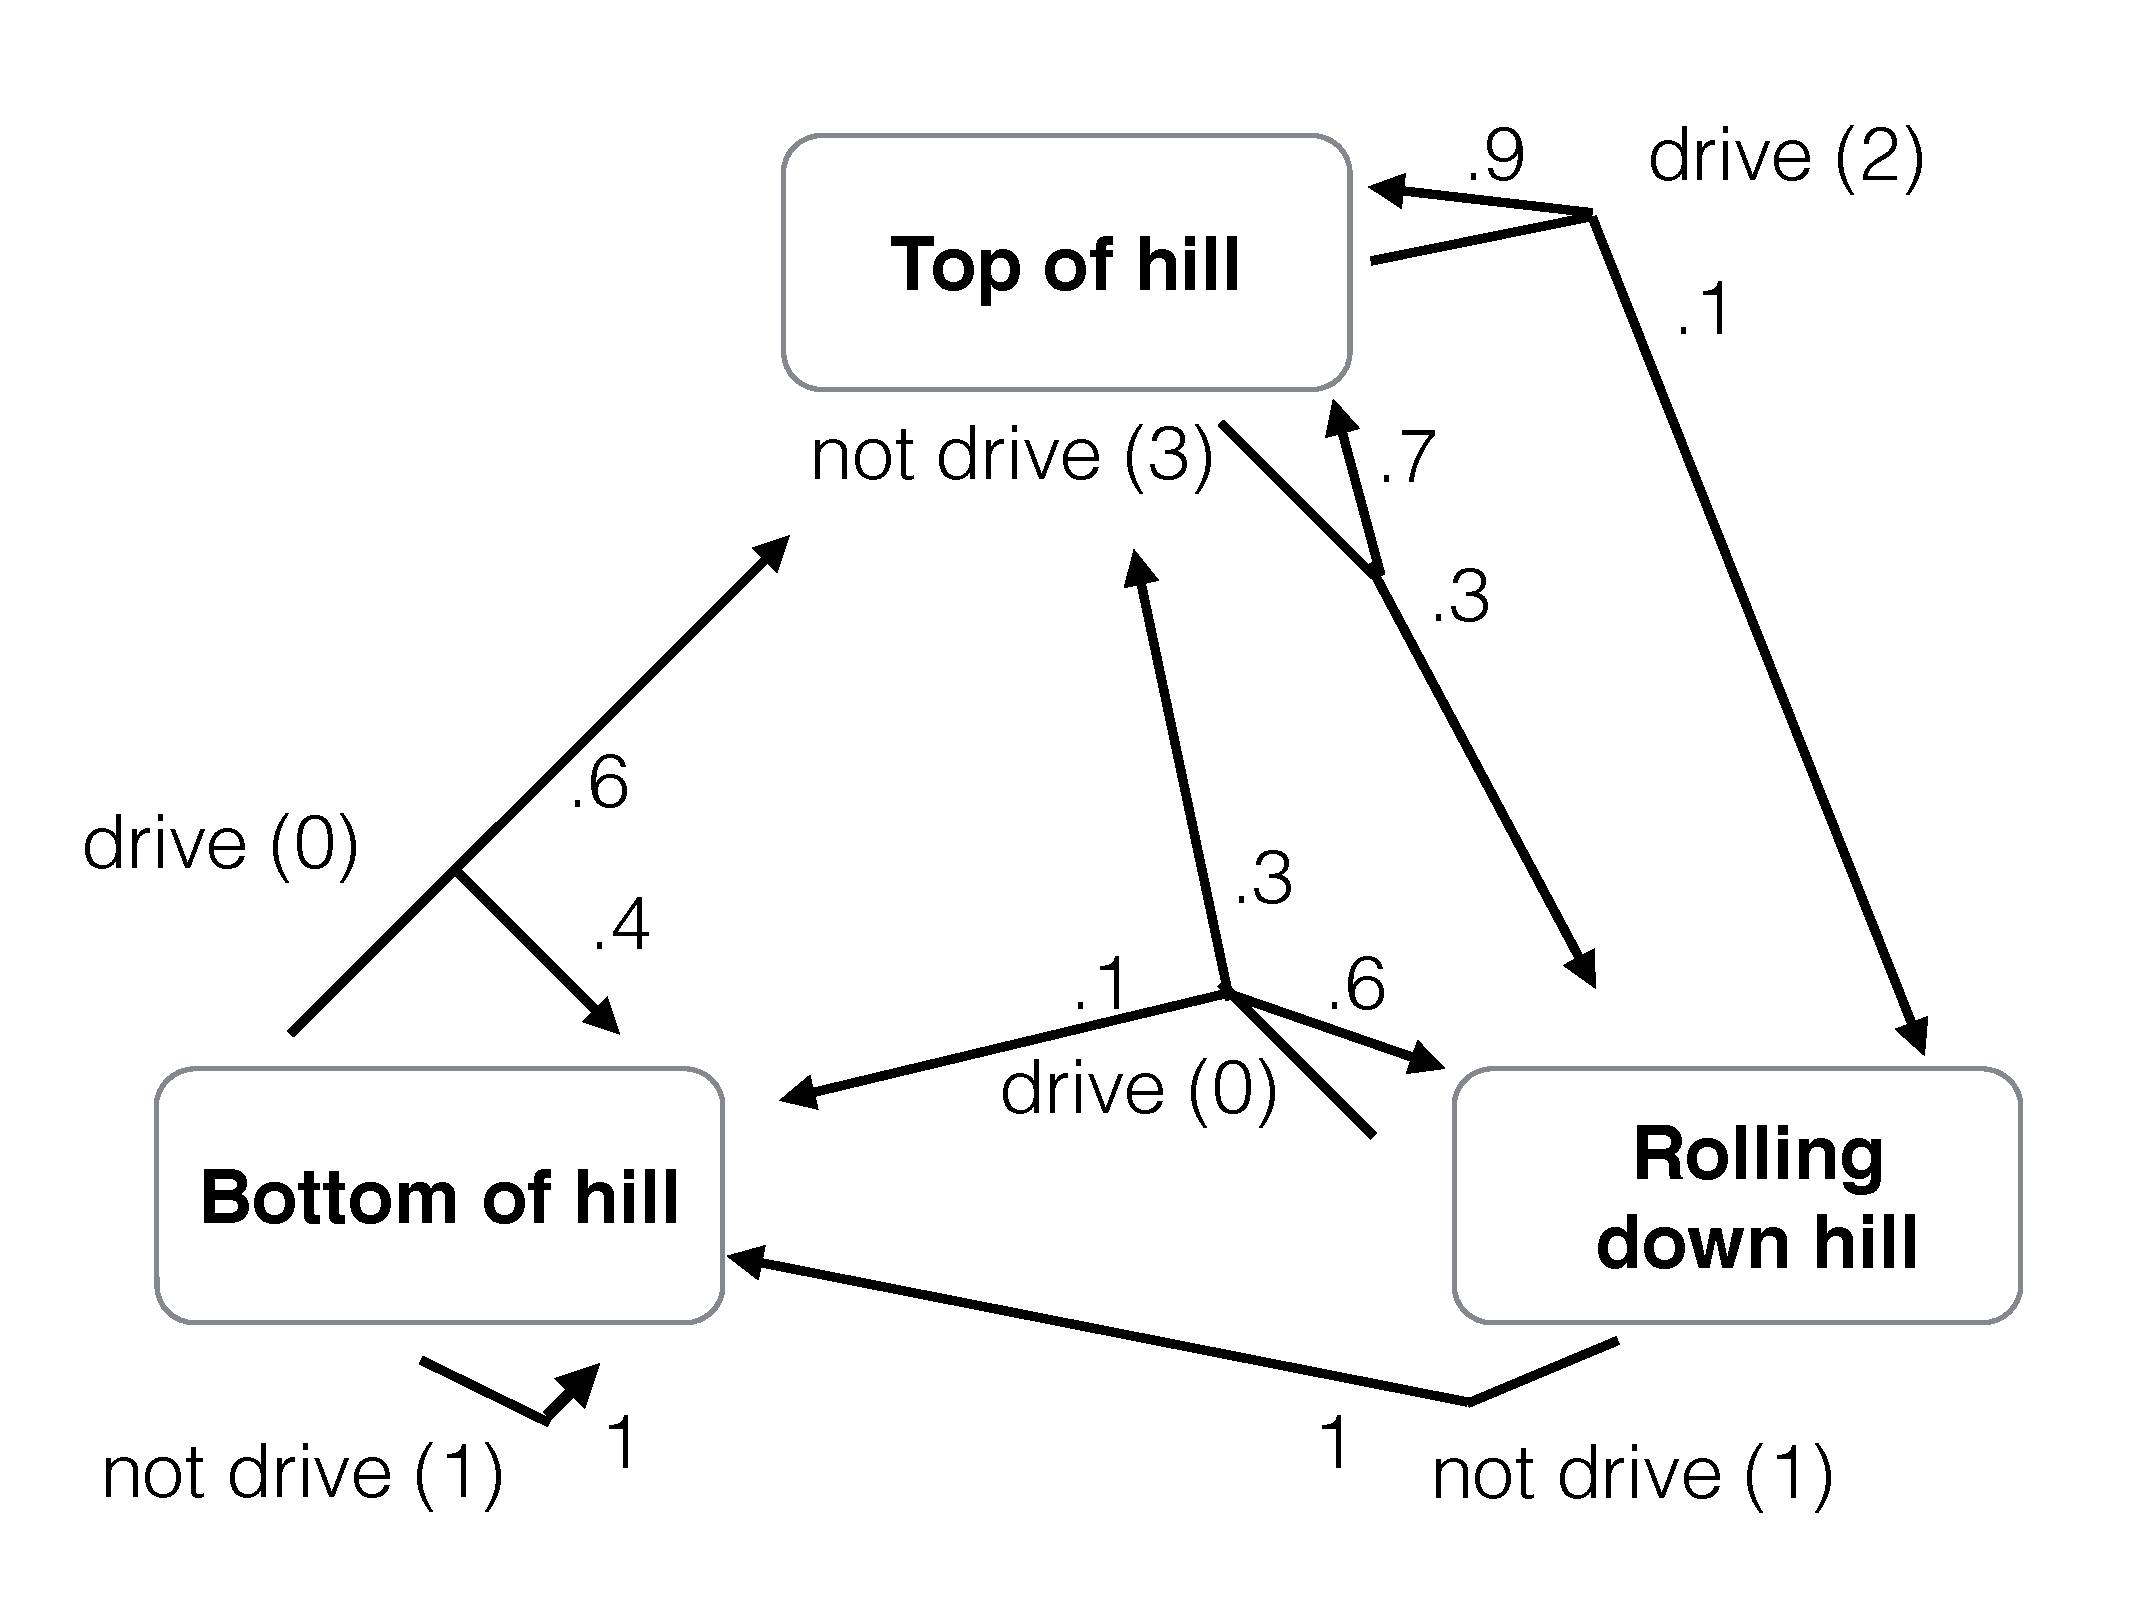
\includegraphics[scale=0.4]{cs570hw5.pdf}
\caption{Graphical MDP}
\end{center}
\end{figure}

I also set up the transition matrices and utilities for each action for use in later problems:

\lstinputlisting[language=R, caption=R Code for Transition Probabilities and Utilities, firstline=6, lastline=44, firstnumber=1]{cs570hw5.r}


\end{answer}




\begin{answer}{2}

My $\mathcal{R}$ code for value iteration is shown below. The values were initialized to zero. The policy recommended does not change after the fourth iteration, but it took five iterations for the values to become stable. 

\lstinputlisting[language=R, caption=R Code for Value Iteration, firstline=51, lastline=73, firstnumber=41]{cs570hw5.r}


The recommended policy is as follows:

\begin{table}[h!]
\begin{center}
\begin{tabular}{c|c}
State & Best action \\
\hline
Top of hill & Not drive \\
Rolling down hill & Not drive \\
Bottom of hill & Drive \\
\end{tabular}
\end{center}
\end{table}


The long-run value of not driving when at the top of the hill is about 7.05 after the fifth iteration. The long-run value of driving when rolling down the hill is about 3.35 after the fifth iteration. The long-run value of driving when at the bottom of the hill is 3.91.

\end{answer}


\begin{answer}{3}

When solving for the optimal policy using policy iteration, we arrive at the same policy as in (2) after three iterations but the values are not the same until the fourth iteration (it took until the fifth iteration in Problem 2 because $v_0$ was initialized to zero rather than the values of the ``not driving'' policy). The best policy in the last two rounds ($v_0$ and $v_1$) is ``never drive'' but the optimal long-run policy is:

\begin{table}[h!]
\begin{center}
\begin{tabular}{c|c}
State & Best action \\
\hline
Top of hill & Not drive \\
Rolling down hill & Not drive \\
Bottom of hill & Drive \\
\end{tabular}
\end{center}
\end{table}

and again the values are 7.05 at the top of the hill, 3.35 when rolling down the hill, and 3.91 at the bottom of the hill.

The $\mathcal{R}$ code for policy iteration is very similar to value iteration, with the addition of a matrix $a$ to keep track of the \texttt{argmax} at each iteration:

\lstinputlisting[language=R, caption=R Code for Policy Iteration, firstline=84, lastline=111, firstnumber=64]{cs570hw5.r}

\end{answer}


\begin{answer}{4}

\paragraph{Changing discount factor}

Decreasing $\delta$ to $\delta=0.5$ changes the optimal policy to ``never drive, regardless of the state.'' When the future is discounted at this rate (i.e. we care more about the present than in the example given in the homework), there is less incentive to expend energy trying to get back to the top of the hill. The long-run equilibrium of this strategy is to remain at the bottom of the hill, content to receive 1 unit of energy per time period.

\paragraph{Changing transition probabilities}

If we change the transition probabilities for ``not drive'' in the ``rolling down the hill'' state so that $p(s^{\prime} = \text{rolling} | a = \text{not drive} ~\&~ s=\text{rolling})=1$, the optimal policy becomes ``not drive if at the top of the hill, and drive if rolling or at the bottom of the hill.'' This makes sense intuitively, because if we get stuck rolling down the hill unless we drive, it makes sense to drive and have a chance of getting back to the top of the hill (where we glean the most energy). 

\paragraph{Changing reward for an action}

I propose changing the reward for not driving when at the bottom of the hill from 1 to 3. The optimal policy would then become ``never drive, regardless of the state.'' Intuitively this makes sense, because if the rover can obtain as much energy at the bottom of the hill as it can at the top there is no reason to expend effort trying to stay at (or relocate to) the top of the hill.


\end{answer}

\end{document}
